

%% AP Style MC Question Archive
%%--------------------------------------------------


%% Conservation of Energy without Friction
%%--------------------------------------------------
\element{ap}{
\begin{question}{energy-without-friction-q01}
    Base your answer to the following question on the picture below which shows a \SI{3}{\kilo\gram} block sliding \SI{50}{\meter} down a frictionless inclined plane dropping a distance of \SI{30}{\meter}.
    \begin{center}
    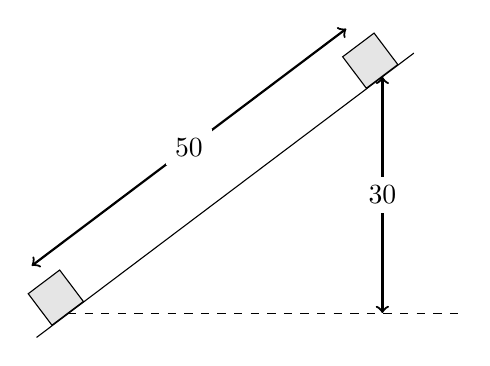
\begin{tikzpicture}
        %% Plane
        \draw (0,0) -- (37:6);
        %% Blocks
        \node[draw,rotate=37,anchor=south,minimum size=0.5cm,fill=white!90!black] (A) at (37:0.5) {};
        \node[draw,rotate=37,anchor=south,minimum size=0.5cm,fill=white!90!black] (B) at (37:5.5) {};
        %% Lables
        \draw[<->,thick] (A.north) ++(127:0.25) -- ++(37:5) node[pos=0.5,anchor=center,fill=white] {\SI{50}{\meter}};
        \draw[<->,thick] (37:5.5) --++(270:3) node[fill=white,pos=0.5,anchor=center] {\SI{30}{\meter}};
        \draw[dashed] (37:0.5) -- ++(0:5);
    \end{tikzpicture}
    \end{center}
    What is the kinetic energy of the block at the end of the drop?
    \begin{multicols}{3}
    \begin{choices}
        \wrongchoice{\SI{90}{\joule}}
        \wrongchoice{\SI{300}{\joule}}
        \wrongchoice{\SI{500}{\joule}}
      \correctchoice{\SI{900}{\joule}}
        \wrongchoice{\SI{1500}{\joule}}
    \end{choices}
    \end{multicols}
\end{question}
}

\element{ap}{
\begin{question}{energy-without-friction-q02}
    A \SI{5}{\kilo\gram} object slides \SI{100}{\meter} down a frictionless inclined plane dropping \SI{45}{\meter}.
    It then slides along a horizontal surface with a coefficient of kinetic friction of \num{0.75} until it stops.
    How long does it take to stop after it leaves the inclined plane?
    \begin{multicols}{3}
    \begin{choices}
        \wrongchoice{\SI{3.0}{\second}}
      \correctchoice{\SI{4.0}{\second}}
        \wrongchoice{\SI{6.0}{\second}}
        \wrongchoice{\SI{12.0}{\second}}
        \wrongchoice{\SI{15.0}{\second}}
    \end{choices}
    \end{multicols}
\end{question}
}

\element{ap}{
\begin{question}{energy-without-friction-q03}
    %Base your answer to the following question on the information below.
    A \SI{4.0}{\kilo\gram} block rests at the edge of a platform that is \SI{20}{\meter} above level ground.
    The block is launched horizontally with an initial velocity of \SI{15}{\meter\per\second}.
    The object's kinetic energy when it hits the ground is most nearly
    \begin{multicols}{3}
    \begin{choices}
        \wrongchoice{\SI{450}{\joule}}
        \wrongchoice{\SI{800}{\joule}}
        \wrongchoice{\SI{1050}{\joule}}
      \correctchoice{\SI{1250}{\joule}}
        \wrongchoice{\SI{2450}{\joule}}
    \end{choices}
    \end{multicols}
\end{question}
}

\element{ap}{
\begin{question}{energy-without-friction-q04}
    A man standing a certain height above the ground throws a rock straight up with an initial velocity of \SI{10}{\meter\per\second}.
    A few moments later,
        the rock hits the ground with a kinetic energy of \SI{450}{\joule}.
    If the man threw this rock horizontally with an initial velocity of \SI{10}{\meter\per\second} at the same height,
        how much kinetic energy would it have just before it hits the ground?
    \begin{multicols}{3}
    \begin{choices}
        \wrongchoice{\SI{50}{\joule}}
        \wrongchoice{\SI{100}{\joule}}
      \correctchoice{\SI{450}{\joule}}
        \wrongchoice{\SI{800}{\joule}}
        \wrongchoice{\SI{950}{\joule}}
    \end{choices}
    \end{multicols}
\end{question}
}

\element{ap}{
\begin{question}{energy-without-friction-q05}
    A man standing a certain height above the ground throws a rock of mass \SI{1}{\kilo\gram} straight up with an initial velocity of \SI{10}{\meter\per\second}.
    A few moments later,
        the rock hits the ground with a kinetic energy of \SI{450}{\joule}.
    If the man dropped this rock from rest,
        how much kinetic energy would it have right before it hits the ground?
    \begin{multicols}{3}
    \begin{choices}
        \wrongchoice{\SI{100}{\joule}}
        \wrongchoice{\SI{200}{\joule}}
        \wrongchoice{\SI{300}{\joule}}
      \correctchoice{\SI{400}{\joule}}
        \wrongchoice{\SI{500}{\joule}}
    \end{choices}
    \end{multicols}
\end{question}
}

%\element{ap}{
%\begin{question}{energy-without-friction-q06}
%    %% Base your answer to the following question on the following information.
%    Two balls of different masses are set at a height of \SI{3}{\meter} above the ground on a frictionless table.
%    The ball on the left is of mass $2M$ and the ball on the right has a mass of $3M$.
%    They both are released simultaneously and slide onto the part of the table \SI{2}{\meter} above the ground.
%    \begin{center}
%    \begin{tikzpicture}
%        %% NOTE: this is a wierd diagram
%        %% TODO: draw tikz
%    \end{tikzpicture}
%    \end{center}
%    What is the total energy of the system?
%    \begin{multicols}{3}
%    \begin{choices}
%        \wrongchoice{$+1 Mg$}
%        \wrongchoice{$+5M g$}
%        \wrongchoice{$+10 Mg$}
%      \correctchoice{$+15 Mg$}
%        \wrongchoice{$+20 Mg$}
%    \end{choices}
%    \end{multicols}
%\end{question}
%}

\element{ap}{
\begin{question}{energy-without-friction-q07}
    %% Base your answer to the following question on the diagram below.
    In the diagram, a box of mass $m$ is sliding down a frictionless ramp of length $L$ with an incline of $\theta$ to the horizontal.
    The mass takes $t$ seconds to slide down the ramp.
    \begin{center}
    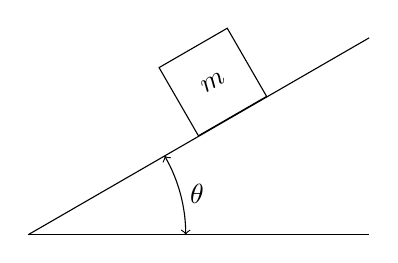
\begin{tikzpicture}
        %% Block and Plane
        \draw (0,0) -- (30:5);
        \draw (0,0) -- (0:4.33);
        \node[anchor=south,draw,rotate=30,minimum size=1cm] (A) at (30:3) {$m$};
        %% angle
        \draw[<->] (2,0) arc (0:30:2) node[pos=0.5,anchor=west] {$\theta$};
    \end{tikzpicture}
    \end{center}
    If released from rest at the top,
        the velocity of the block at the bottom of the ramp will be:
    \begin{multicols}{2}
    \begin{choices}
        \wrongchoice{$gLt\sin\theta$}
        \wrongchoice{$gL\sin\theta$}
        \wrongchoice{$\sqrt{gt\sin\theta}$}
      \correctchoice{$\sqrt{2gL\sin\theta}$}
        \wrongchoice{$\sqrt{gL\sin\theta}$}
    \end{choices}
    \end{multicols}
\end{question}
}

\element{ap}{
\begin{question}{energy-without-friction-q08}
    A crate with mass $m$ slides down a frictionless ramp with length $L$ and vertical height $h$.
    The crate's change in kinetic energy from the top to the bottom is equal to:
    \begin{multicols}{2}
    \begin{choices}
        \wrongchoice{$\dfrac{mL^2}{2}$}
        \wrongchoice{$\dfrac{-mL^2}{2}$}
        \wrongchoice{$-mgh$}
      \correctchoice{$mgh$}
        \wrongchoice{Cannot be determined from the information given.}
    \end{choices}
    \end{multicols}
\end{question}
}

\element{ap}{
\begin{question}{energy-without-friction-q09}
    A block with a mass of \SI{10}{\kilo\gram} slides down a frictionless inclined plane of length \SI{25}{\meter} and height \SI{20}{\meter}.
    It's speed at the bottom is most nearly:
    \begin{multicols}{3}
    \begin{choices}
        \wrongchoice{\SI{15}{\meter\per\second}}
      \correctchoice{\SI{20}{\meter\per\second}}
        \wrongchoice{\SI{30}{\meter\per\second}}
        \wrongchoice{\SI{37}{\meter\per\second}}
        \wrongchoice{\SI{45}{\meter\per\second}}
    \end{choices}
    \end{multicols}
\end{question}
}

\element{ap}{
\begin{question}{energy-without-friction-q10}
    An object with a mass of \SI{4}{\kilo\gram} is released from rest at the top of a ramp with length \SI{10}{\meter} that makes an angle of \ang{30} with the horizontal.
    The coefficient of kinetic friction between the block and the ramp is \num{0.4}.
    The speed the block will have when it has traveled \SI{5}{\meter} down the ramp is most nearly:
    \begin{multicols}{3}
    \begin{choices}
      \correctchoice{\SI{3.9}{\meter\per\second}}
        \wrongchoice{\SI{5.6}{\meter\per\second}}
        \wrongchoice{\SI{7}{\meter\per\second}}
        \wrongchoice{\SI{7.9}{\meter\per\second}}
        \wrongchoice{\SI{10.4}{\meter\per\second}}
    \end{choices}
    \end{multicols}
\end{question}
}

\element{ap}{
\begin{question}{energy-without-friction-q11}
    An object is falling from a height of $h$ in a vacuum and reaches a final velocity of $v$.
    When the object has fallen a distance of $h/2$,
        its velocity is:
    \begin{multicols}{3}
    \begin{choices}
      \correctchoice{$\dfrac{v}{\sqrt{2}}$}
        \wrongchoice{$\dfrac{v}{2}$}
        \wrongchoice{$\dfrac{v}{4}$}
        \wrongchoice{$\sqrt{2}v$}
        \wrongchoice{$4v$}
    \end{choices}
    \end{multicols}
\end{question}
}

\element{ap}{
\begin{question}{energy-without-friction-q12}
    %% Base your answer to the following question on the following situation.
    An object weighing \SI{10}{\newton} swings at the end of a rope that is \SI{0.72}{\meter} long as a simple pendulum.
    At the bottom of the of the swing,
        the tension in the string is \SI{12}{\newton}.
    What is the maximum height above its lowest point that the object reaches?
    \begin{multicols}{3}
    \begin{choices}
        \wrongchoice{\SI{0.036}{\meter}}
        \wrongchoice{\SI{0.060}{\meter}}
      \correctchoice{\SI{0.072}{\meter}}
        \wrongchoice{\SI{0.144}{\meter}}
        \wrongchoice{\SI{0.360}{\meter}}
    \end{choices}
    \end{multicols}
\end{question}
}

\element{ap}{
\begin{questionmult}{energy-without-friction-q13}
    Units of energy include which of the following?
    \begin{choices}
        %% ANS is 3
      \correctchoice{Newton meter (\si{\newton\meter})}
        \wrongchoice{Ampere volt (\si{\ampere\volt})}
      \correctchoice{Volt coulomb (\si{\volt\coulomb})}
    \end{choices}
\end{questionmult}
}

\element{ap}{
\begin{question}{energy-without-friction-q14}
    A student throws a stone upward at an angle of \ang{30}.
    Which statement best describes the stone at the highest point that it reaches?
    \begin{choices}
        \wrongchoice{Its acceleration is zero.}
        \wrongchoice{Its acceleration is at a maximum.}
        \wrongchoice{Its potential energy is at a minimum.}
      \correctchoice{Its kinetic energy is at a minimum.}
        \wrongchoice{Its potential and kinetic energies are equal}
    \end{choices}
\end{question}
}

\element{ap}{
\begin{questionmult}{energy-without-friction-q15}
    Units of energy include which of the following?
    \begin{choices}
        %% ANS is 3
      \correctchoice{Joule (\si{\joule})}
      \correctchoice{Ampere volt per second (\si{\ampere\volt\per\second})}
      \correctchoice{Volt coulomb (\si{\volt\coulomb})}
    \end{choices}
\end{questionmult}
}

\element{ap}{
\begin{question}{energy-without-friction-q16}
    Tarzan of mass $m_1$ swings from a height of $h$ on a vine.
    When potential energy is at its minimum,
        he picks up Jane (mass $m_2$).
    What height will the Tarzan-Jane system reach when its potential energy reaches a maximum?
    \begin{multicols}{2}
    \begin{choices}
        \wrongchoice{$h\left(m_1+m_2\right)$}
      \correctchoice{$\dfrac{m_1 h}{m_1+m_2}$}
        \wrongchoice{$\dfrac{m_1+m_2}{2hm_2}$}
        \wrongchoice{$\dfrac{m_1+m_2}{2hm_1}$}
        \wrongchoice{$2hm_1$}
    \end{choices}
    \end{multicols}
\end{question}
}

\element{ap}{
\begin{question}{energy-without-friction-q17}
    Tarzan (\SI{90}{\kilo\gram}) carries Jane (\SI{55}{\kilo\gram}) with one arm while swinging on a vine.
    They began at a height of \SI{15}{\meter}.
    If Tarzan drops Jane when their kinetic energy is a maximum,
        how high will Tarzan swing?
    \begin{multicols}{3}
    \begin{choices}
        \wrongchoice{\SI{20}{\meter}}
      \correctchoice{\SI{24}{\meter}}
        \wrongchoice{\SI{27}{\meter}}
        \wrongchoice{\SI{31}{\meter}}
        \wrongchoice{\SI{35}{\meter}}
    \end{choices}
    \end{multicols}
\end{question}
}

%\newcommand{\apEnergyWithoutFrictionQEighteen}{
%\begin{tikzpicture}
%    %% NOTE: complex graph
%    %% TODO: draw tikz/pgfplots
%\end{tikzpicture}
%}
%
%\element{ap}{
%\begin{question}{energy-without-friction-q18}
%    %% Base your answers to questions 18 through 22 on the diagram below which shows a frictionless track
%    \begin{center}
%        \apEnergyWithoutFrictionQEighteen
%    \end{center}
%    At which point would an object at rest be in unstable equilibrium?
%    \begin{multicols}{2}
%    \begin{choices}[o]
%        \wrongchoice{$A$}
%        \wrongchoice{$B$}
%        \wrongchoice{$C$}
%      \correctchoice{$D$}
%        \wrongchoice{$E$}
%    \end{choices}
%    \end{multicols}
%\end{question}
%}
%
%\element{ap}{
%\begin{question}{energy-without-friction-q19}
%    %% Base your answers to questions 18 through 22 on the diagram below which shows a frictionless track
%    \begin{center}
%        \apEnergyWithoutFrictionQEighteen
%    \end{center}
%    At which point is an object at rest in stable equilibrium?
%    \begin{multicols}{2}
%    \begin{choices}[o]
%        \wrongchoice{$A$}
%      \correctchoice{$B$}
%        \wrongchoice{$C$}
%        \wrongchoice{$D$}
%        \wrongchoice{$E$}
%    \end{choices}
%    \end{multicols}
%\end{question}
%}
%
%\element{ap}{
%\begin{question}{energy-without-friction-q20}
%    %% Base your answers to questions 18 through 22 on the diagram below which shows a frictionless track
%    \begin{center}
%        \apEnergyWithoutFrictionQEighteen
%    \end{center}
%    If an object is released at the beginning of the track,
%        which of the following is true at point $E$?
%    \begin{choices}
%        \wrongchoice{It is in static equilibrium}
%        \wrongchoice{It is losing kinetic energy}
%      \correctchoice{It is in dynamic equilibrium}
%        \wrongchoice{There is a net force acting on the object}
%        \wrongchoice{Its kinetic energy is \SI{25}{\joule}}
%    \end{choices}
%\end{question}
%}
%
%\element{ap}{
%\begin{question}{energy-without-friction-q21}
%    %% Base your answers to questions 18 through 22 on the diagram below which shows a frictionless track
%    \begin{center}
%        \apEnergyWithoutFrictionQEighteen
%    \end{center}
%    Which of the following best describes the motion of an object as it approaches point $B$,
%        if it was released from rest at the beginning of the track?
%    \begin{choices}
%        \wrongchoice{It is losing potential energy only.}
%        \wrongchoice{It is gaining kinetic energy only.}
%        \wrongchoice{It is gaining potential energy and gaining kinetic energy}
%      \correctchoice{It is losing potential energy and gaining kinetic energy}
%        \wrongchoice{It is gaining heat energy, gaining kinetic energy, and losing potential energy}
%    \end{choices}
%\end{question}
%}
%
%\element{ap}{
%\begin{question}{energy-without-friction-q22}
%    %% Base your answers to questions 18 through 22 on the diagram below which shows a frictionless track
%    \begin{center}
%        \apEnergyWithoutFrictionQEighteen
%    \end{center}
%    If an object of mass \SI{5}{\kilo\gram} is released from rest at the beginning of the track,
%        what is its velocity at point $D$?
%    \begin{multicols}{3}
%    \begin{choices}
%        \wrongchoice{\SI{1}{\meter\per\second}}
%        \wrongchoice{\SI{1.4}{\meter\per\second}}
%      \correctchoice{\SI{2}{\meter\per\second}}
%        \wrongchoice{\SI{2.2}{\meter\per\second}}
%        \wrongchoice{\SI{3}{\meter\per\second}}
%    \end{choices}
%    \end{multicols}
%\end{question}
%}


\endinput


